% Physics in the Household

\documentclass[11pt]{article}

\usepackage[a4paper, margin=1in]{geometry}

\usepackage{amsmath}

\usepackage{amssymb}

\usepackage[german]{babel}

\usepackage[autostyle=true]{csquotes}

\usepackage{libertine}

\usepackage[libertine]{newtxmath}

\usepackage{tikz}

\usepackage{gensymb}

\usepackage{fancyhdr}

\usepackage{amsfonts}

\usepackage{pgfplots}

\pgfplotsset{compat=1.10}

\usepackage{multicol}

\usepackage{caption}

\usepackage{floatrow}

\everymath{\displaystyle}

% Header / footer settings

\pagestyle{fancy}
\fancyhf{}
\renewcommand{\headrulewidth}{0.2mm}
\fancyhead[C]{Funktionen}
\renewcommand{\footrulewidth}{0.2mm}
\fancyfoot[L]{Peter Goldsborough}
\fancyfoot[C]{\thepage}
\fancyfoot[R]{\today}

\fancypagestyle{plain}{%
	\fancyhf{}
	\renewcommand{\headrulewidth}{0mm}%
	\renewcommand{\footrulewidth}{0.2mm}%
	\fancyfoot[L]{Peter Goldsborough}
	\fancyfoot[C]{\thepage}
	\fancyfoot[R]{\today}
}


\setlength{\headheight}{15pt}

\setlength{\parindent}{0pt}

\addtolength{\parskip}{\baselineskip}


\newcommand{\overbar}[1]{\mkern 1.5mu\overline{\mkern-1.5mu#1\mkern-1.5mu}\mkern 1.5mu}

\newcommand{\heading}[1]{\begin{center}\Huge \textbf{#1}\end{center}\par}

\newcommand{\sub}[1]{\vspace{\parskip}{\LARGE\textbf{#1}}}

\newcommand{\subsub}[1]{{\Large \textbf{#1}}}

\newcommand{\subsubsub}[1]{\textbf{#1}}

\newcommand{\colvec}[1]{\begin{pmatrix}#1\end{pmatrix}}

\newcommand{\extrapar}{\par\vspace{\baselineskip}}

\newcommand{\zitat}[1]{\foreignquote{german}{#1}}

\newcommand{\bolditem}[1]{\item \textbf{#1}}

\newcommand{\titleitem}[1]{\bolditem{#1}\par}

\newcommand{\defas}{ \dots \,\,}

\begin{document}
\thispagestyle{plain}

\heading{Physics in the Household}

\sub{Electrical Safety Precautions}

\subsub{Wires}

Power supplies carrying current to and from household appliances commonly consist of three wires: a \emph{live} wire, a \emph{neutral} wire and an \emph{earthing} wire. Current flows from the mains through the live wire to the appliance, and flows back to the mains through the neutral wire. The earthing wire (usually colored green or yellow), provides a low resistance path to ground (earth). This earthing wire is usually connected to (touches) the casing of the appliance such that, were a fault to occur and current from the live wire somehow be able to flow through the case, it would be directed to earth safely without causing any harm to the user. This is especially important when the case is made of a conductive material such as metal, while it is needed less for plastic covers. Consider the situation of a hairdryer being used in a moist or wet environment such as a bathroom. It may occur that some water happens to provide a conductive path between the current flowing through the live wire and the casing of the hairdryer, which moreover may be made of a metallic material. Were there no earthing wire to provide a low-resistance path for the current to flow to ground, the current would flow through the next-best path to ground: the person using the hairdryer. The result is that the person receives an electrical shock. This is why the earthing is a highly important component of any appliance's wiring. 

To ensure that electric current flows through a wire as safely as possible, minimizing the possible damage to humans handling the wires, all wires are \emph{insulated}. In fact, there are two layers of insulation: \emph{functional} insulation and \emph{protective} insulation. Each of the three wires described above, the neutral, live and earthing wire, is insulated individually to prevent the copper wires from touching (which may lead to a short circuit). The second, outer layer of insulation --- the \emph{protective} insulation --- solely protects the wires from outside influences. 

\begin{plot}
	
	% Protective insulation
	\draw [very thick, orange] (0, 0) circle [radius=1cm];

	% Protective insulation label
	\draw [<-, orange]
	      (0, -1.1) -- ++(0, -1) node [below] {Protective insulation};

	% Live wire
	\draw [fill=brown, very thick] (-0.45, -0.3) circle [radius=0.4];

	% Live wire label
	\draw [<-] (-0.45, -0.3) -- ++(-1, 0) node [left] {Live Wire};

	% Neutral wire
	\draw [fill=cyan, very thick] (0.45, -0.3) circle [radius=0.4];

	% Neutral wire label
	\draw [<-] (0.45, -0.3) -- ++(1, 0) node [right] {Neutral Wire};

	% Earthing wire
	\draw [fill=green, very thick] (0, 0.5) circle [radius=0.4];

	% Earthing wire label
	\draw [<-] (0, 0.5) -- ++(0, 1) node [above] {Earthing Wire};

	% Functional isolation label
	\draw [red, ->] (-3, 1) node [above] {Functional Isolation} -- (-0.8, 0);

\end{plot}

\sub{Fuses}

Fuses are thin pieces of metal that are added to power supplies and in other areas within a household, that open a circuit in case of a short circuit or current overload (e.g. from too many devices drawing too much current from a power supply). The working principle of such fuses is simply that they melt when the current strength is too high, typically around 20 Amperes. Thus, you should check the fuses of your electricity box if your oven or stove suddenly goes out. It and all other appliances connected to the same power outlet may have been drawing too much current.

\sub{Residual Current Circuit Brakers}

A Residual Current Circuit Braker (RCCB) is an electrical device typically found in your home's electricity box, that is used to interrupt an electric circuit in case of a fault in an appliance or due to any other current leakage (such as when current from the live wires flows to ground through a human instead of the neutral wire).

\begin{figure}[h!]
	\centering
	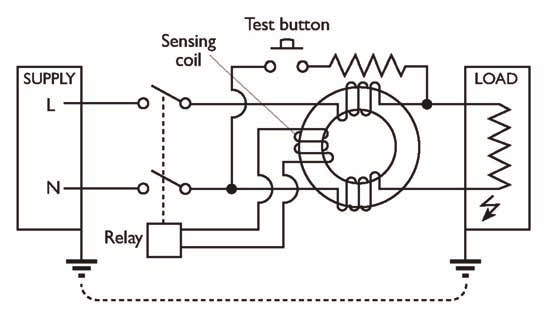
\includegraphics[scale=0.7]{img/rccb}
\end{figure}

Under normal conditions, the alternating current flowing through the live wire towards the load generates an alternating magnetic field around and within the first coil wrapped around the soft iron ring. This alternating magnetic field causes the magnetic flux within the soft iron ring to change with time and would, if this were the end of the story, induce an alternating voltage within the \emph{sensing coil}. However, if all goes well and there is no fault and current leakage in the load, the same alternating current from the live wire also flows through the neutral wire with the same strength and thus through the secondary coil on the lower end of the soft iron ring. This secondary coil has the same number of turns and is wound in the same way as the primary coil, such that the magnetic field generated in the secondary coil will equal the magnetic field produced in the first in terms of strength and magnitude, but will be phase shifted 180\degree{} or $\pi$ radians due to the way they are wound (in the same way). As a result, under normal conditions, the magnetic field will phase cancel and thus there will be no change in magnetic flux to induce a voltage in the sensing coil. 

However, if there is a fault in the appliance to which the live and neutral wire are connected, some or all of the current may not end up flowing back through the neutral wire, but to ground via a human or some other path. Consequently, the current flowing through the neutral wire will be less than the original current that was drawn from the load through the live wire and, as a result, the magnetic field produced in the secondary coil on the side of the neutral wire will not equal the magnetic field from the live wire. There will thus be a certain changing magnetic flux experienced by the sensing coil, such that a voltage is induced. This will cause an induced current to flow through the relay, which opens the connections of the live and neutral wire. Thus, the circuit would be broken and no more current would flow to ground in any way that it normally shouldn't. This happens very quickly, as RCCBs typically react within milliseconds and detect current strength differences as small as 10 milli-amperes. 

To test if the RCCB is working, the test button may be used. The resistance in the test circuit is lower than the resistance of the load, such that the charges flowing will prefer the path of less resistance and flow through the test circuit and not to the load. However, the alternating current will already have generated an alternating magnetic field in the coil connected to the live wire. As there can be no magnetic field produced by the secondary coil (on the neutral side), the magnetic field from the live wire is not cancelled and induces a voltage and current in the sensing coil. This will open the circuit and stop the flow of current. Nevertheless, the test button should be pressed only for a very short time, as the strong current flowing through the relatively small resistance of the test button will cause it to become hot quite quickly.  

\sub{Effects of Electric Shocks}

The degree to which an electric shock harms a person depends on three main factors, listed below. In general, an electric shock may cause burns due to current locally heating the skin and fibrilation --- the rapid and irregular contraction of muscle fibers. The main distinction between direct and alternating current in this case is the fact that direct current causes a constant stimulus to be experienced by muscles, while alternating current sends new stimuli many times a second, e.g. 100 times per second in case of the usual 50 Hz AC current from any household mains supply. Another important term in connection with electric shocks is the \emph{let-go-current} (``Loslassschwelle''). At this current value --- around 10mA --- it becomes very hard to let go of the source of the electric shock. Lastly, it should be said that what is known as a \emph{clinical shock} results in a weak pulse as well as irregular breathing.

\begin{itemize}

	\item The \textbf{duration} of the shock. The longer the duration, the greater the damage.

	\item The \textbf{current strength} $I$ flowing through the body for the duration of the shock. As the current $I$ is directly proportional to voltage $U$ --- assuming a constant resistance $R$ (as defined by Ohm's law: $I = \frac{U}{R}$) --- a high voltage indicates a higher risk for producing high currents.

	\item The \textbf{frequency} of the current, as alternating current can excite nerves that control muscles, causing burns from the heating of the skin. 
\end{itemize}

\begin{plot}
	
	% Current axis
	\draw [->] (0, 0) -- (10, 0) node [above] {Current $I$};

	% Current labels
	\draw (-2, -0.5) \foreach \i in {$100\mu A$, 1mA, 10mA, 100mA, 1A, 10A}
	{
		 ++(2, 0) node {\i}
	};

	% Duration axis
	\draw [->] (0, 0) -- (0, 6) node [right] {Duration $T$};

	% Duration labels
	\draw (-0.7, -{6/3}) \foreach \i in {10ms, 100ms, 1s, 10s}
	{
		 ++(0, {6/3}) node {\i}
	};

	% Zone 1, border
	\draw (2, 0) -- ++(0, 5.5);

	% Zone 1, label
	\draw (1, 3) node [rotate=90] {No sensation};

	% Zone 2, border
	\draw (4, 5.5) .. controls (4.5, 3) .. (7, 0);

	% Zone 2, label
	\draw (4.1, 0.5) node {Perception without harm};

	% Let-go-current
	\draw [red] (4, 0) -- ++(0, 5.5)
	      node [midway, rotate=90, above] {Let-Go-Current};

	% Zone 3, border
	\draw (5, 5.5) .. controls (5, 2) and (8, 5) .. (7, 0);

	% Zone 3, label
	\draw (5.6, 3) node [rotate=-50] {Muscle Contractions};

	% Zone 4, label
	\draw (8, 4) node {High Danger};

\end{plot}

\end{document}